\documentclass{article}
\usepackage{amsmath}
\usepackage{enumerate}
\usepackage{listings}
\usepackage{moreverb}
\usepackage[margin=1in]{geometry}
\usepackage{graphicx}
\usepackage{dsfont}
\title{STA 360: Assignment 8}
\author{Michael Lin}

\begin{document}
\maketitle

\begin{enumerate}[8.1]
\setcounter{enumi}{2}
\item
\begin{enumerate}[(a)]
\item Below are plots of $\sigma^2, \mu, \tau^2$ for 3 different runs.

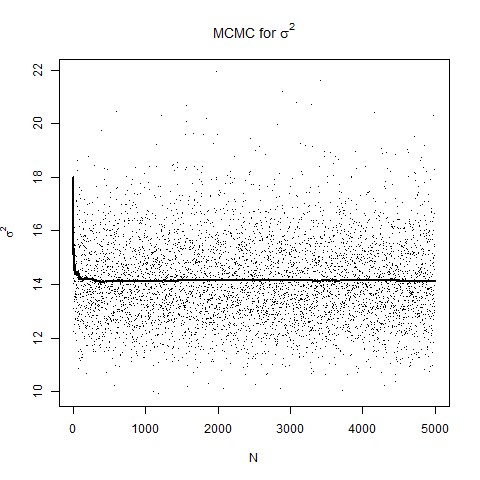
\includegraphics[scale = 0.3]{sig.png}
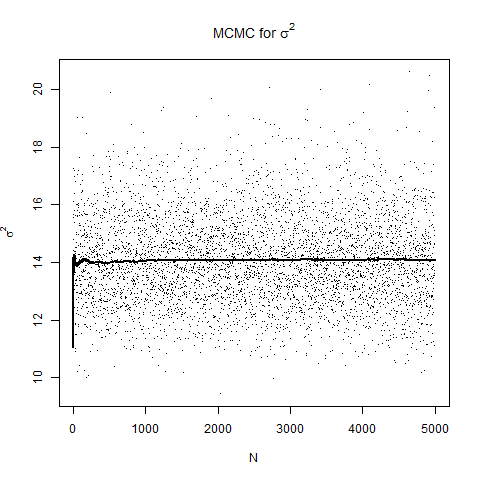
\includegraphics[scale = 0.3]{sig-a.png}
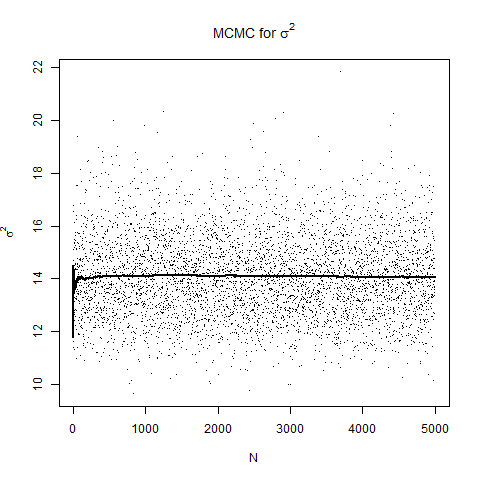
\includegraphics[scale = 0.3]{sig-b.png}\\

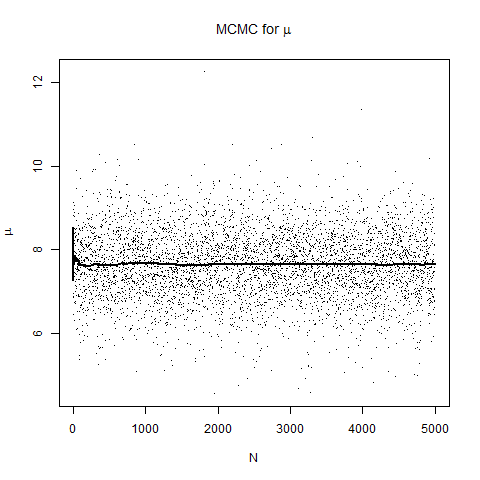
\includegraphics[scale = 0.3]{mu.png}
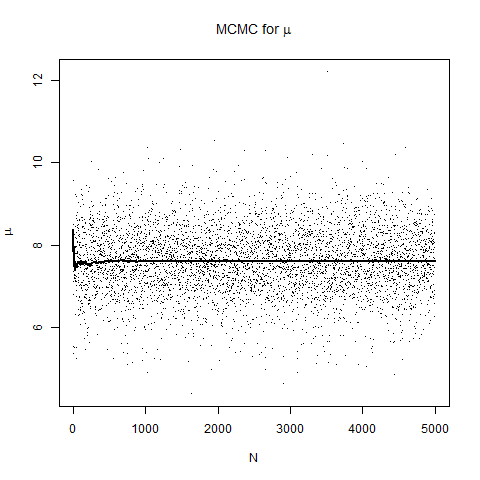
\includegraphics[scale = 0.3]{mu-a.png}
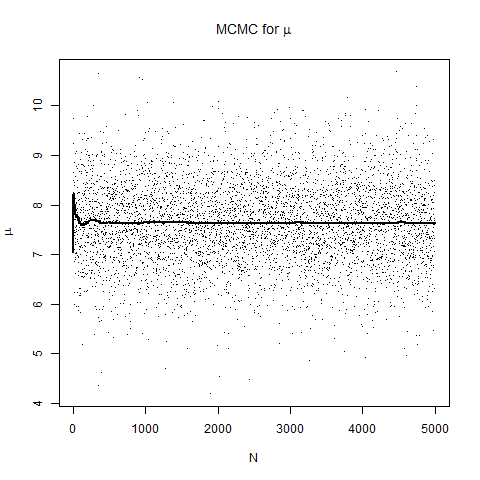
\includegraphics[scale = 0.3]{mu-b.png}\\

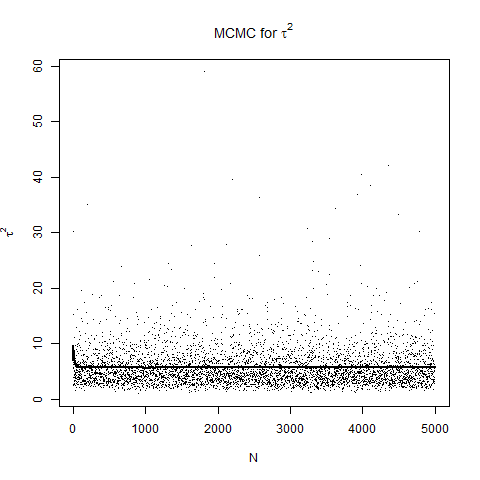
\includegraphics[scale = 0.3]{tau.png}
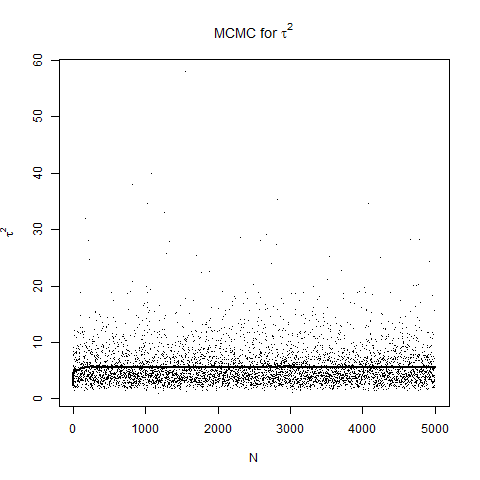
\includegraphics[scale = 0.3]{tau-a.png}
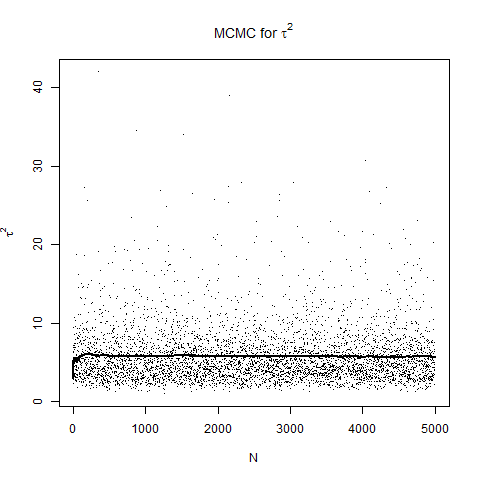
\includegraphics[scale = 0.3]{tau-b.png}\\

\pagebreak
\item Posterior means and 95\% confidence regions:
\begin{center}

\begin{tabular}{l|l|l}
 & Posterior Mean & 95\% Credible Interval \\ \hline
 $\sigma^2$ & 14.0755 & [11.32467, 17.49859] \\ \hline
 $\mu$ & 7.645934 & [6.065964, 9.204791] \\ \hline
 $\tau^2$ & 5.640306 & [1.950527, 15.128655]
\end{tabular}
\end{center}

Plots of prior and posterior densities are also shown below:

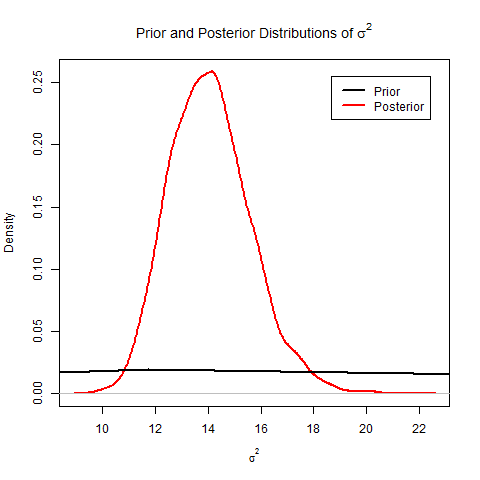
\includegraphics[scale = 0.3]{sig-density.png}
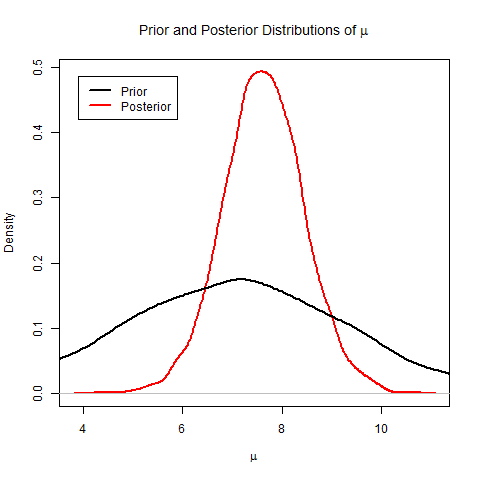
\includegraphics[scale = 0.3]{mu-density.png}
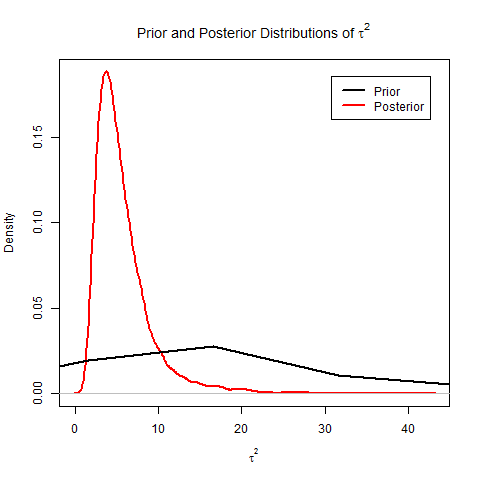
\includegraphics[scale = 0.3]{tau-density.png} \\

The data allowed us to obtain posterior distributions with smaller spread than the respective prior distributions. In particular, the prior distribution of $\sigma^2$ is uninformative while its posterior distribution suggests a mean of around 14. The posterior mean of $\mu$ is greater than prior mean while the posterior mean of $\tau^2$ is slightly less than the corresponding prior mean. This implies that the mean of all observations is the variance between groups is larger than prior belief while the population variance is slightly smaller than prior belief.

\item Defining $R$ as follows:
$$R = \frac{\tau^2}{\sigma^2 + \tau^2} $$
below is a plot of the prior and posterior density of $R$:

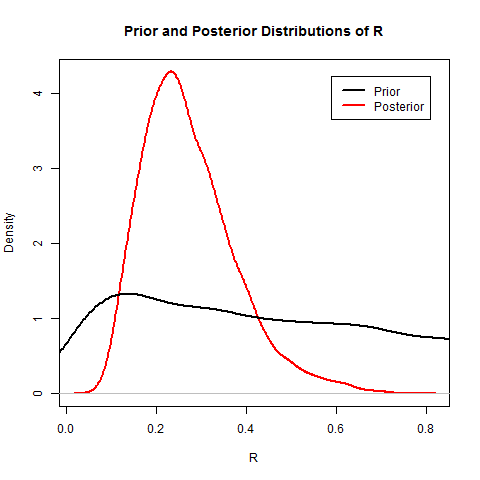
\includegraphics[scale = 0.5]{rplot.png}

The prior for R is close to a uniform distribution, which suggested little prior belief that between-school variation differs from within-school variation. However, the posterior distribution has most of the mass around 0.2 and 0.4, which suggests that there is less variance between groups than within groups.

\item The posterior probability that $\theta_7$ is smaller than $\theta_6$ is 0.6006. The posterior probability that $\theta_7$ is the smallest of all the $\theta$'s is 0.339.

\item Below is a plot of the sample averages $\bar{y}_1,\dots,\bar{y}_8$ against the posterior expectations $\theta_1, \dots, \theta_8$:

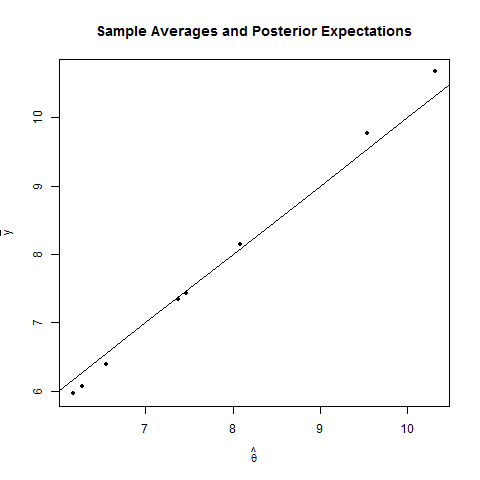
\includegraphics[scale = 0.5]{groupmean.png}

The plot demonstrates the effect of shrinkage: smaller-than-average $\bar{y}$ values are predicted to have slightly higher predicted means, while the opposite is true for larger-than-average $\bar{y}$ values. In other words, the slope of the line passing through the data points is greater than the slope of the line shown. The sample mean of all observations is 7.766628, which is slightly larger than the posterior mean of $\mu$ which is 7.645934.

\end{enumerate}

\end{enumerate}

\pagebreak
R code for 8.3:
\listinginput[1]{1}{assign8.r}

\end{document}